\documentclass[11pt,a4paper]{article}
\usepackage[T1]{fontenc}
\usepackage{iftex}
\ifPDFTeX\usepackage[utf8]{inputenc}\fi
\usepackage{lmodern}
\usepackage[margin=27mm]{geometry}
\usepackage{amsmath,amssymb,bm,mathtools}
\usepackage{graphicx,booktabs,microtype}
\usepackage[numbers,sort&compress]{natbib}
\usepackage{xcolor}
\usepackage[colorlinks=true,allcolors=blue!45!black]{hyperref}
\usepackage{placeins}
\usepackage[font=small,labelfont=bf]{caption}
\renewcommand{\topfraction}{0.95}
\renewcommand{\bottomfraction}{0.85}
\renewcommand{\textfraction}{0.05}
\renewcommand{\floatpagefraction}{0.75}
\setcounter{totalnumber}{4}
\graphicspath{{figures/}}
\newcommand{\dd}{\mathrm{d}}
\newcommand{\Hc}{\mathcal H}
\newcommand{\Sthree}{\mathbb S^3}
\newcommand{\ph}{\varphi}
\newcommand{\order}{\mathcal O}
% Generated by scripts/reproduce.py; do not edit.
\newcommand{\CoreDensityPercent}{0.3748}
\newcommand{\CoreLapse}{0.99989999}
\newcommand{\CoreClockOffset}{-33.580}
\newcommand{\RadialDelay}{65.536}
\newcommand{\BornDelay}{65.533}
\newcommand{\AngularShift}{146.887}
\newcommand{\BornAngularShift}{146.858}
\newcommand{\CoreRadius}{0.3041}
\newcommand{\CoreMassScaled}{11.8282}
\newcommand{\RemainderPower}{2.000}
\newcommand{\MaxPeculiarSpeed}{189.481}

\title{A Temporal--Radial View of an Expanding Three-Sphere\\with a Localized Mass Perturbation}
\author{Valdemar Rolfsen}
\date{Working draft v0.5 \quad 27 November 2026}
\begin{document}
\maketitle
\begin{abstract}
An observer's sky combines emission events from different cosmic times.
Drawing successive spatial slices as nested spheres makes this distinction
visible: a past-directed light path crosses progressively smaller layers on
an expanding branch. We extend this representation with a reproducible
linear scalar perturbation of a closed, dust-filled FLRW universe. A smooth
potential well, with its homogeneous and dipole components removed, specifies
a localized overdensity and compensating surroundings. The linear Einstein
constraints determine the density and velocity perturbations, and the
potential evolves through the dust perturbation equation. This connects
spatial geometry, normal-observer clock rates, and null propagation in one
specified spacetime approximation. A first-order Euclidean embedding of the
spatial slices produces an outward radial deformation at the potential well,
while the lapse decreases there: spatial deformation and clock slowing
cannot be identified with one ``depth into the past.'' We integrate light
paths, match source worldlines to a fixed reception event, and check timing
changes against an independent first-order integral. These are illustrative
calculations in established general relativity, not an observational fit,
a black-hole model, or a claim of a new gravitational law.
\end{abstract}
\section{Motivation and the question being tested}
The starting picture is a three-dimensional universe represented by the
three-dimensional boundary of a four-dimensional ball. Each layer is a
complete spatial slice at one time. Successively larger layers represent
later stages of expansion. A familiar two-dimensional balloon surface is
a lower-dimensional analogy for this construction.

The important observational object is the \emph{view line}: the image of
a received light ray, traced backward from the observer. Its earlier events
lie on earlier spatial layers. A diagram therefore separates the universe
at a specified time from the collection of emission events visible to an
observer. The physical basis is standard null propagation and cosmological
distance geometry \citep{Hogg1999,DavisLineweaver2004}.

The motivation for a local-mass extension is equally concrete. Can the same
representation show spatial distortion, gravitational time dilation, and
the changes in view lines without assigning conflicting meanings to drawing
radius? We answer this for a controlled linear example. We first specify a
spacetime metric and a consistent matter perturbation. We then derive the
clock and ray equations, and finally choose drawings of those quantities.

This is a reorganization and extension of the v0.4 manuscript. Its core
distinction between light-cone observation and simultaneous separation is
retained. The original text and three figures are preserved in
\texttt{archive/v0.4/}. The earlier proposed Bianchi/vorticity program is
deferred while the local-gravity question is developed. Neither version
establishes a priority claim for polar cosmological diagrams.

\paragraph{Scope.}
The background here is positively curved, simply connected, and expanding
over the plotted interval. It contains pressureless matter and no cosmological
constant. This choice permits explicit calculations; it is not a fit to the
observed universe. The local source is a small, evolving dust overdensity
with compensating surroundings. It is not a star of constant mass, a point
singularity, or a black hole. The distinction is essential when interpreting
the resulting geometry.

\section{Expanding spatial layers and the unperturbed view line}
\label{sec:background}
Let $\gamma_{ij}$ be the metric of a unit three-sphere:
\begin{equation}
 \dd\Omega_3^2=\dd\chi^2+\sin^2\chi\,
 (\dd\theta^2+\sin^2\theta\,\dd\phi^2).
\end{equation}
The closed FLRW metric is
\begin{equation}\label{eq:flrw}
 \dd s^2=-c^2\dd t^2+A^2(t)\dd\Omega_3^2
 =A^2(\eta)(-\dd\eta^2+\dd\Omega_3^2),
 \qquad \dd\eta=\frac{c\,\dd t}{A(t)}.
\end{equation}
Here $A$ has units of length, and $\eta,\chi,\theta,\phi$ are dimensionless.
The time $t$ is background cosmic time; $\eta$ is conformal time.
This is a standard closed spatial geometry \citep{Carroll2004,TongGR}.

A fixed-time slice has the isometric Euclidean embedding
\begin{equation}\label{eq:embedding-background}
 \bm X=A(t)\bm n,\qquad \bm n\in\Sthree\subset\mathbb R^4.
\end{equation}
The nested collection of these slices is a drawing of history. Its Euclidean
radial line element has positive sign, while the time term in
Eq.~\eqref{eq:flrw} has negative sign. Thus the full drawing is not an
isometric Euclidean embedding of Lorentzian spacetime.

For a radial photon received at $\eta_o$ by the observer at $\chi=0$,
\begin{equation}\label{eq:background-ray}
 \chi(\eta)=\eta_o-\eta,\qquad
 \chi(t)=\int_t^{t_o}\frac{c\,\dd t'}{A(t')}.
\end{equation}
The temporal--radial drawing is
\begin{equation}\label{eq:polar-map}
 (X,Y)=A(t)(\cos\chi,\sin\chi).
\end{equation}
Tracing the photon backward decreases $A$ on an expanding branch and
changes $\chi$. Its drawing moves inward \emph{and} across spatial positions.
A straight radius at fixed spatial coordinates represents a comoving
observer's history, not a null ray. The angle $\chi$ in this radial picture
is not an angle on the observer's sky.

\subsection{A background that satisfies the field equations}
For dust with $\Lambda=0$, an exact closed solution is
\begin{equation}\label{eq:dust}
 A(\eta)=A_{\max}\sin^2\!\frac{\eta}{2},\qquad
 ct(\eta)=\frac{A_{\max}}{2}(\eta-\sin\eta),\qquad 0<\eta<\pi.
\end{equation}
We use only this expanding branch. A prime denotes $\dd/\dd\eta$. Define
\begin{equation}\label{eq:hubble}
 \Hc=\frac{A'}{A}=\cot\frac{\eta}{2},\qquad
 \Hc'=-\frac{\Hc^2+1}{2},\qquad H=\frac{c\Hc}{A}.
\end{equation}
The background density $\bar\rho$ is a mass density:
\begin{equation}\label{eq:friedmann}
 \frac{8\pi G}{3c^2}\bar\rho A^2=\Hc^2+1,
 \qquad A(\Hc^2+1)=A_{\max},\qquad \bar\rho A^3=\text{constant}.
\end{equation}
The calculations use $A_{\max}$ as length unit and $A_{\max}/c$ as time
unit. No physical value of either unit is inferred.

\begin{figure}[htbp]
 \centering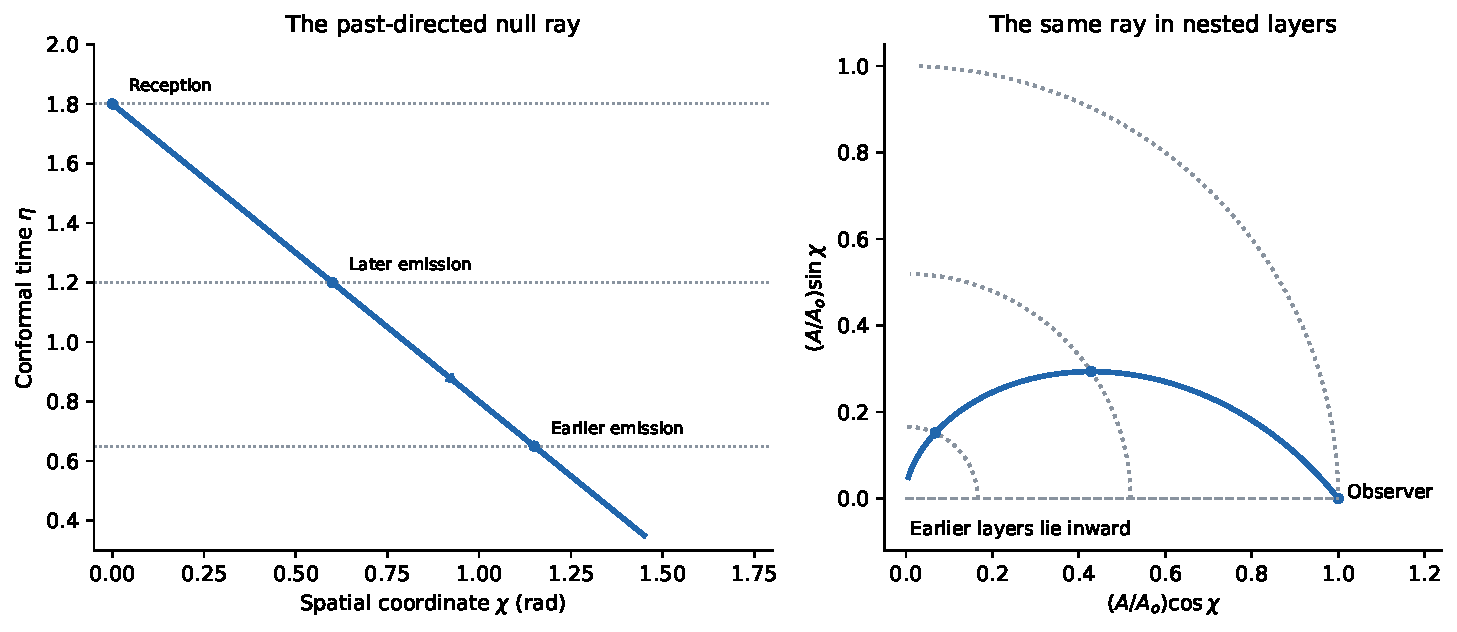
\includegraphics[width=\linewidth]{01-view-lines.pdf}
 \caption{The same closed-dust radial null ray in conformal and
 temporal--radial coordinates. Dotted curves mark corresponding times.
 Radius on the right encodes $A/A_o$; the observer is on the outer layer.
 The formal small-radius limit is not a location on any spatial slice.}
 \label{fig:baseline}
\end{figure}
\FloatBarrier

\section{A localized mass perturbation on the three-sphere}
\label{sec:mass}
In Newtonian (Poisson) gauge, take a scalar perturbation with negligible
anisotropic stress:
\begin{equation}\label{eq:perturbed}
 \dd s^2=A^2(\eta)\left[-(1+2\ph)\dd\eta^2
 +(1-2\ph)\gamma_{ij}\dd x^i\dd x^j\right]+\order(\epsilon^2).
\end{equation}
The potential $\ph=\Phi/c^2$ is dimensionless and of order $\epsilon$.
It perturbs both the lapse and the spatial metric. Curved-background scalar
perturbations are an established way to describe inhomogeneities
\citep{Canay2022}. We specify the source through the linear Einstein
constraints rather than inserting a flat-space $-GM/r$ potential globally.

\subsection{Evolution and reconstructed matter}
The linear dust equation for the potential, with unit positive spatial
curvature, is
\begin{equation}\label{eq:bardeen}
 \ph''+3\Hc\ph'+(2\Hc'+\Hc^2-1)\ph=0.
\end{equation}
The comoving density contrast $\Delta$, velocity potential $V$, and
Newtonian-gauge density contrast $\delta_N$ obey
\begin{align}
 \Delta&=\frac{2}{3(\Hc^2+1)}(\nabla_\gamma^2+3)\ph,
       \label{eq:constraint-density}\\
 V&=-\frac{2}{3(\Hc^2+1)}(\ph'+\Hc\ph),
       \label{eq:constraint-velocity}\\
 \delta_N&=\Delta+3\Hc V.\label{eq:constraint-gauge}
\end{align}
These are the first-order dust relations, specialized to the conventions
above \citep[Eq.~(14b)--(16)]{UgglaWainwright2013}. Our convention for the
dimensionless peculiar velocity is $v^i/c=\nabla_\gamma^i V$ at this order.
Using Eq.~\eqref{eq:hubble} directly verifies
\begin{equation}\label{eq:conservation}
 V'+\Hc V=-\ph,\qquad \delta_N'=-\nabla_\gamma^2V+3\ph'.
\end{equation}
The accompanying symbolic script checks both identities without selecting
one particular spatial eigenmode.

Write $\ph(\eta,\chi)=\epsilon g(\eta)F(\cos\chi)$, with $g(\eta_o)=1$.
Equation~\eqref{eq:bardeen} reduces for Eq.~\eqref{eq:dust} to
\begin{equation}\label{eq:growth}
 g''+3\cot(\eta/2)g'-2g=0.
\end{equation}
We select the regular growing solution by starting with a multiple of
\begin{equation}\label{eq:growth-series}
 1+\frac{\eta^2}{7}+\frac{\eta^4}{84}+\frac{\eta^6}{1320}
 +\order(\eta^8)
\end{equation}
at $\eta_i=10^{-3}$, and normalize at reception. An independent numerical
check uses the reduction-of-order expression
\begin{equation}
 g(\eta)\propto \frac{\Hc(\eta)}{A^2(\eta)}
 \int_0^\eta\frac{A(\tilde\eta)}{\Hc^2(\tilde\eta)}\,\dd\tilde\eta.
\end{equation}

\subsection{Smoothness, compensation, and the low spatial modes}
Let $\mu=\cos\chi$ and $\kappa=\sigma^{-2}$. Define
\begin{align}
 Q(\mu)&=\exp[\kappa(\mu-1)],\\
 q_0&=\langle Q\rangle=\frac{2e^{-\kappa}I_1(\kappa)}{\kappa},
 &q_1&=4\langle\mu Q\rangle=\frac{8e^{-\kappa}I_2(\kappa)}{\kappa},\\
 F(\mu)&=-\frac{Q(\mu)-q_0-q_1\mu}{1-q_0-q_1}.
 \label{eq:profile}
\end{align}
Here $I_n$ is the modified Bessel function and the normalized three-sphere
average of a radial function is
\begin{equation}
 \langle f\rangle=\frac{2}{\pi}\int_0^\pi f(\cos\chi)\sin^2\chi\,\dd\chi.
\end{equation}
Since $\langle\mu^2\rangle=1/4$, this construction gives
$F(1)=-1$, $\langle F\rangle=0$, and $\langle\mu F\rangle=0$.
It removes the homogeneous mode and the rotationally symmetric dipole
mode, avoiding a background redefinition and the exceptional lowest
scalar modes. Smoothness at both poles follows from smooth dependence
on $\cos\chi$.

The sphere Laplacian is computed without singular polar divisions:
\begin{equation}\label{eq:laplace}
 \nabla_\gamma^2F=(1-\mu^2)F_{,\mu\mu}-3\mu F_{,\mu}.
\end{equation}
For the specified parameters, Eq.~\eqref{eq:constraint-density} has a
positive central core and negative surrounding regions. Its integral
over the entire background three-sphere vanishes. The localized mass
is therefore an excess relative to the homogeneous dust distribution,
with compensation; it is not extra net mass added to an unchanged
compact background. The broad tail from the low-mode removal is included
in all calculations.

For a quantitative mass label, define the positive-core excess using
the comoving density contrast and background volume element:
\begin{equation}\label{eq:mass}
 M_+(\eta)=4\pi\bar\rho A^3
 \int_0^{\chi_c}\Delta(\eta,\chi)\sin^2\chi\,\dd\chi,
\end{equation}
where $\chi_c$ is the first zero of $\Delta$. This is a specified linear
background-relative mass diagnostic, not a nonlinear quasi-local mass.
Its evolving value is appropriate to growing dust structure.

\section{Spatial deformation and elapsed time}
\label{sec:geometry}
\subsection{Clock rates require the lapse}
For observers held at fixed spatial coordinates, Eq.~\eqref{eq:perturbed}
gives
\begin{equation}\label{eq:lapse}
 \dd\tau=\frac{A}{c}\sqrt{1+2\ph}\,\dd\eta
 =(1+\ph)\dd t+\order(\epsilon^2).
\end{equation}
A negative potential reduces the elapsed proper time relative to the
chosen background-time interval. To first order the accumulated change
at a fixed coordinate position is
\begin{equation}\label{eq:clock-offset}
 \delta\tau(\chi)=\frac{1}{c}\int_{\eta_1}^{\eta_2}
 A(\eta)\ph(\eta,\chi)\,\dd\eta.
\end{equation}
The normal observers used here need not follow the perturbed dust flow:
the latter has velocity from Eq.~\eqref{eq:constraint-velocity}.
Clock comparisons across separated worldlines require specified events
and a synchronization or signal protocol. Equation~\eqref{eq:clock-offset}
states explicitly which coordinate endpoints are being compared; it is
not a claim of an absolute local cosmic age.

\subsection{A spatial embedding has a different sign}
At fixed $\eta$, an approximate radial embedding in Euclidean four-space is
\begin{equation}\label{eq:deformed-embedding}
 \bm X(\eta,\bm n)=A(\eta)[1-\ph(\eta,\bm n)]\bm n.
\end{equation}
Because $\bm n\cdot\dd\bm n=0$, its induced line element is
\begin{align}
 \dd\bm X\cdot\dd\bm X
 &=A^2\left[(1-\ph)^2\dd\Omega_3^2+(\dd\ph)^2\right]\\
 &=A^2(1-2\ph)\dd\Omega_3^2+\order(\epsilon^2).
 \label{eq:induced}
\end{align}
Thus it reproduces the spatial metric to first order for a fixed smooth
profile as $\epsilon\to0$. Gradients must also be controlled: for narrow
profiles, discarded terms scale as $\epsilon^2/\sigma^2$ rather than
simply $\epsilon^2$ with a width-independent coefficient.

At the core $\ph<0$, Eq.~\eqref{eq:deformed-embedding} produces an
\emph{outward} deformation, while Eq.~\eqref{eq:lapse} produces slower
clocks. This is a result of this particular first-order spatial embedding
and time slicing; it is not a universal rule that mass must bulge outward
in every embedding diagram. It does show why the rubber-sheet ``dent''
cannot simultaneously be assumed to measure earlier cosmic time.

The intrinsic spatial-curvature perturbation provides another way to
describe the distortion:
\begin{equation}\label{eq:spatial-curvature}
 {}^{(3)}R=\frac{6}{A^2}
 +\frac{4}{A^2}(\nabla_\gamma^2+3)\ph+\order(\epsilon^2).
\end{equation}
It is the scalar curvature of the specified spatial slices. Its
perturbation, like the slices themselves, depends on the chosen slicing.
It is distinct from the extrinsic appearance of a curve on a page.

\begin{figure}[htbp]
 \centering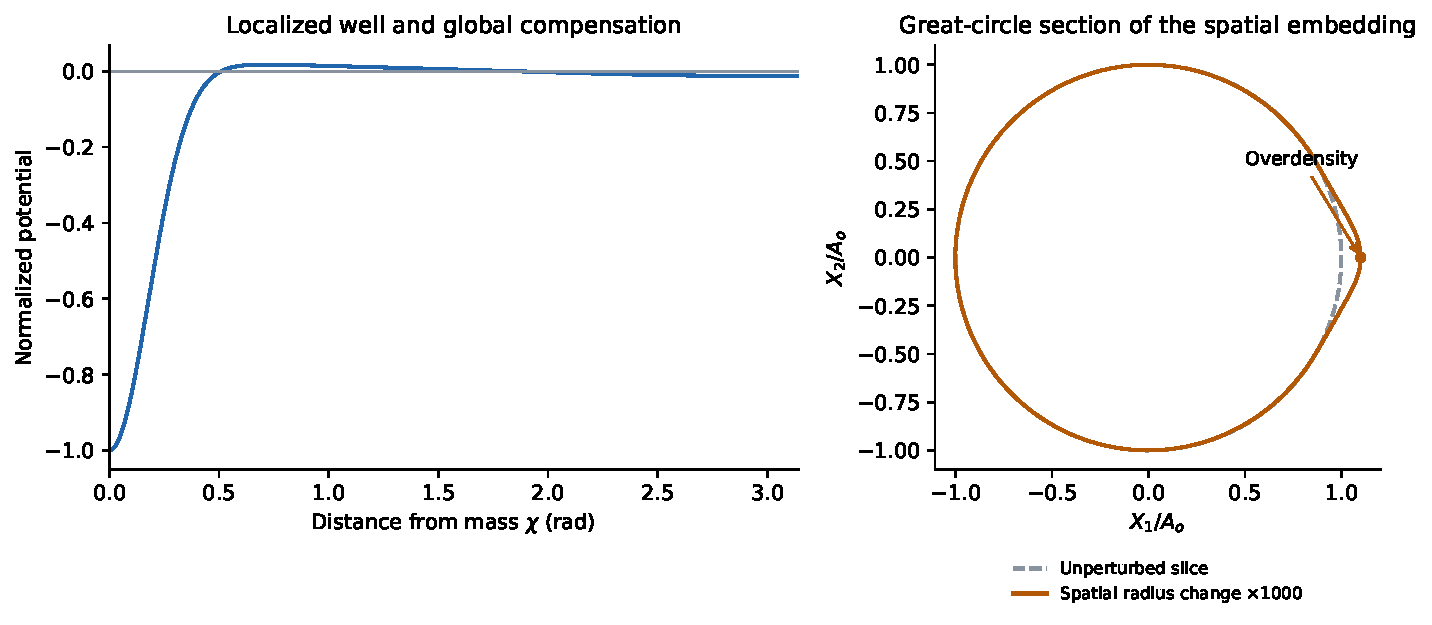
\includegraphics[width=\linewidth]{02-spatial-deformation.pdf}
 \caption{The potential profile at reception and a great-circle section
 of Eq.~\eqref{eq:deformed-embedding}. The plotted radial deformation is
 amplified by a factor of 1000 to make its sign visible. The amplified
 curve is illustrative, not an isometric embedding at the displayed
 amplitude. The physical fractional radius change at the core is $10^{-4}$.}
 \label{fig:deformation}
\end{figure}
\begin{figure}[htbp]
 \centering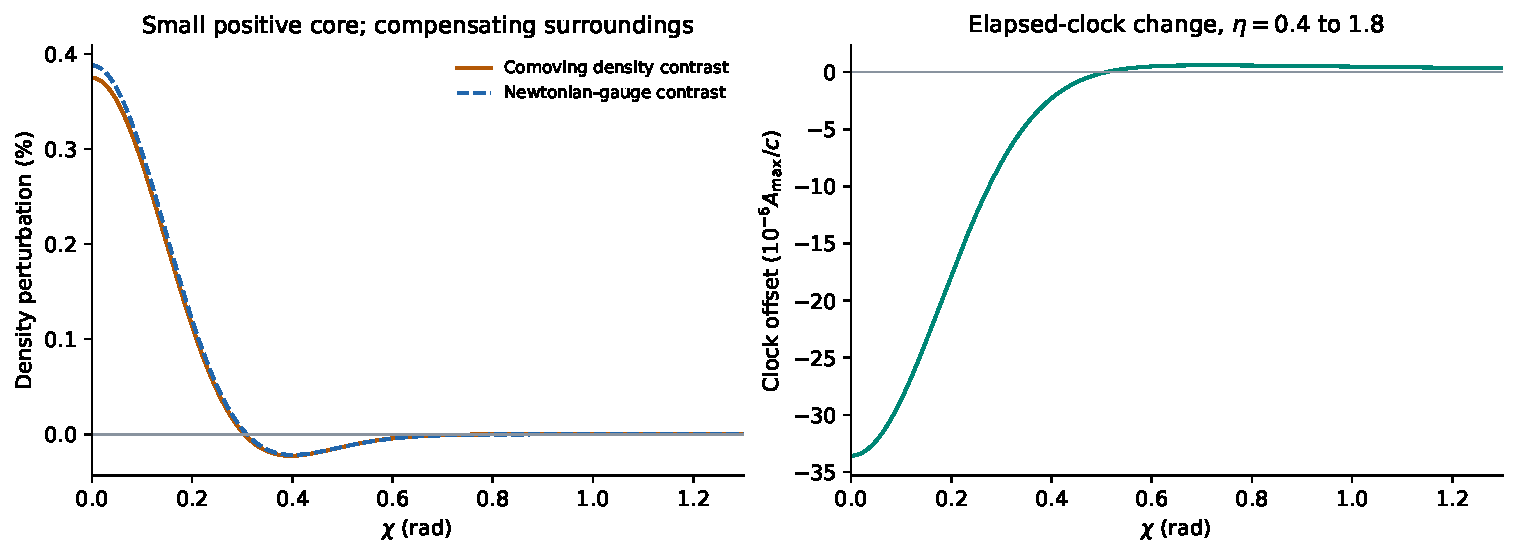
\includegraphics[width=\linewidth]{03-density-and-clocks.pdf}
 \caption{The density contrasts and the accumulated first-order
 normal-observer clock offset. Both follow from the same potential.
 The clock interval uses fixed background conformal times, and the
 surrounding density compensation is part of the model.}
 \label{fig:clocks}
\end{figure}

\section{View lines, deflection, and timing}
\label{sec:rays}
\subsection{Null propagation in the specified metric}
For numerical ray tracing define
\begin{equation}\label{eq:optical}
 N=\sqrt{1+2\ph},\qquad B=\sqrt{1-2\ph},\qquad
 v=\frac{N}{B}=1+2\ph+\order(\epsilon^2).
\end{equation}
The symbol $v$ is a dimensionless coordinate speed per conformal time on
the unit sphere. The speed measured locally by an orthonormal observer
remains $c$. The code treats the displayed truncated metric as its
numerical metric. Taking square roots and integrating its trajectories
retains some terms of order $\epsilon^2$ and higher, but does not promote
it to an exact solution of the nonlinear Einstein equations. All physical
claims are restricted to first order.

Set $s=\eta_o-\eta$. Spherical symmetry about the mass confines each
spatial ray to a totally geodesic two-sphere in $\Sthree$. Represent this
two-sphere by $\bm n\in\mathbb R^3$, with
$\bm n^2=1$ and tangent momentum $\bm p\cdot\bm n=0$. The mass lies
at $\bm n_L=(1,0,0)$, so $\mu=\bm n\cdot\bm n_L$.
The reduced optical Hamiltonian is $\mathcal K=v|\bm p|$. In the
past-directed parameter and with momentum pointing along the past
spatial trajectory, its equations are
\begin{align}
 \frac{\dd\bm n}{\dd s}&=v\frac{\bm p}{|\bm p|},\label{eq:ray-n}\\
 \frac{\dd\bm p}{\dd s}&=-|\bm p|\nabla_S v-v|\bm p|\bm n,
 \label{eq:ray-p}\\
 \nabla_Sv&=\frac{2v}{1-4\ph^2}\,
 \epsilon g F_{,\mu}(\bm n_L-\mu\bm n).
 \label{eq:gradient}
\end{align}
The last term in Eq.~\eqref{eq:ray-p} preserves tangency to the unit
sphere. These equations preserve $\bm n^2=1$, $\bm n\cdot\bm p=0$,
and the angular momentum component about the lens axis. Conformal time
is not an affine parameter.

The physical ray is displayed using the \emph{background-time} map
$\bm X_{
\mathrm{view}}=A(\eta)\bm n(\eta)$, which keeps radius exclusively as
the time-layer label. Figure~\ref{fig:nested} uses this map.
Equation~\eqref{eq:deformed-embedding}, used separately for spatial
deformation, has a different purpose. The two maps are explicitly
distinguished instead of silently assigning both meanings to one radius.

\subsection{A deflection with fixed endpoints}
Comparing arbitrary curves at equal coordinate parameters is insufficient
to define a lensing prediction. We fix a coordinate-stationary source
worldline, an observer worldline, and a reception event. For the reference
FLRW ray, choose a launch angle $\alpha_0$ in the observer's tangent frame
and a source distance $s_0$. Its source position is
\begin{equation}
 \bm n_s=\cos s_0\,\bm n_o+\sin s_0\,\bm e_o(\alpha_0).
\end{equation}
For the perturbed ray, a two-variable shooting calculation adjusts
$(\alpha,s)$ until the same spatial source is reached. The emission time
is allowed to change because the source is a worldline, not a fixed
emission event. The predicted angular displacement is
\begin{equation}\label{eq:angular-shift}
 \delta\alpha=\alpha-\alpha_0.
\end{equation}
The angular coordinate in the observer's tangent plane equals the
orthonormal-frame angle because the spatial metric there is conformally
isotropic. Consequently Eq.~\eqref{eq:angular-shift} is an astrometric
model-to-reference prediction for the stipulated source matching. It is
not inferred from the apparent winding of a polar drawing.

The sources and observer in this experiment are test worldlines held at
fixed coordinates. They are not assumed to follow the dust velocity
field. Using dust tracers would require evolving their positions and
including their peculiar-velocity contributions.

An independent first-order check follows by projecting the perturbed ray
onto the parallel-transported transverse unit vector $\bm b$ along its
reference great circle. The transverse displacement obeys
$y''+y=-2\bm b\cdot\nabla_S\ph$, with the derivatives here taken
with respect to $s$. Setting $y(0)=y(s_0)=0$ gives
\begin{equation}\label{eq:born-angle}
 \delta\alpha_{\mathrm{first}}=\frac{2}{\sin s_0}
 \int_0^{s_0}\sin(s_0-s)\,
 \bm b\cdot\nabla_S\ph(\eta_o-s,\bm n_0(s))\,\dd s.
\end{equation}
The test remains away from $s_0=\pi$, where antipodal focusing would
invalidate this simple boundary-value comparison.

\subsection{An independent radial timing calculation}
A ray through the center follows a meridian with no transverse deflection.
Let $\ell$ be its unwrapped spatial arc coordinate. The null condition
gives $\dd\ell/\dd s=v$. For a fixed source arc distance $s_0$, expand
the arrival condition $\ell(s)=s_0$ to first order about the background
path $\bm n_0(\ell)$:
\begin{equation}\label{eq:born-delay}
 \Delta s=-2\int_0^{s_0}
 \ph(\eta_o-\ell,\bm n_0(\ell))\,\dd\ell+\order(\epsilon^2).
\end{equation}
This is an additional conformal lookback at fixed reception, relative to
the matched FLRW source. A negative potential along most of the path
gives $\Delta s>0$: the emission must occur earlier. The corresponding
background cosmic-time difference is computed with Eq.~\eqref{eq:dust}.
Raw conformal-time differences depend on the specified coordinate and
background identification. An operational clock delay would additionally
specify the emission/reception clock protocol.

\subsection{Frequency along a view line}
For the coordinate-stationary normal observers, the photon energy is
proportional to $|\bm p|/(AB)$. Thus
\begin{equation}\label{eq:redshift}
 1+z=\frac{|\bm p_e|}{|\bm p_o|}\frac{A_oB_o}{A_eB_e}.
\end{equation}
The normalization of $\bm p$ cancels. At $\epsilon=0$, this reduces to
$1+z=A_o/A_e$, checked numerically. For moving sources or receivers,
the appropriate four-velocities must instead be used in
$(k_\mu u^\mu)_e/(k_\mu u^\mu)_o$. The present calculation includes
the metric's gravitational and expansion effects for the stated normal
observers, and omits dust Doppler terms.

\section{Reproducible numerical example}
\label{sec:results}
The default experiment uses
\begin{equation}
 \epsilon=10^{-4},\quad\sigma=0.18,\quad\eta_o=1.8,\quad
 \chi_o=0.65,\quad s_0=1.3.
\end{equation}
The unperturbed emission time is $\eta_e=0.5$.
The main nonradial comparison uses $\alpha_0=0.25$ radians.
The entire background interval is expanding; no ray crosses a turnaround.
The largest Newtonian-gauge density contrast at reception is below
$0.4\%$. The sampled maximum peculiar speed is
$\MaxPeculiarSpeed\times10^{-6}c$. Both the matter perturbations and
the potential remain small in this experiment.

\begin{table}[htbp]
 \centering\small
 \begin{tabular}{@{}p{0.65\linewidth}r@{}}
 \toprule
 Quantity & Computed value\\
 \midrule
 Core comoving density contrast & $\CoreDensityPercent\%$\\
 Core lapse $N_o$ & $\CoreLapse$\\
 Positive-core radius $\chi_c$ (rad) & $\CoreRadius$\\
 $GM_+/(c^2A_{\max})$, in units of $10^{-6}$ & $\CoreMassScaled$\\
 Core clock offset, in units of $10^{-6}A_{\max}/c$ & $\CoreClockOffset$\\
 Radial additional lookback $\Delta s$, in units of $10^{-6}$ & $\RadialDelay$\\
 First-order integral for $\Delta s$, in units of $10^{-6}$ & $\BornDelay$\\
 Matched-source angular shift at $\alpha_0=0.25$ ($\mu$rad) & $\AngularShift$\\
 First-order angular integral ($\mu$rad) & $\BornAngularShift$\\
 Fitted power of the timing remainder versus $\epsilon$ & $\RemainderPower$\\
 \bottomrule
 \end{tabular}
 \caption{Illustrative dimensionless results, generated directly from
 the calculation. These are not measurements or predictions for an
 identified astronomical object. The clock interval is $0.4\leq\eta\leq1.8$.}
 \label{tab:results}
\end{table}

The positive-core mass uses Eq.~\eqref{eq:mass}. Since its value depends
on the source evolution and the specified density contrast, it should
not be interpreted as a conserved Schwarzschild mass.
The ray integrator agrees with the independent radial integral through
first order. Varying $\epsilon$ from $2.5\times10^{-5}$ to
$4\times10^{-4}$ gives a remainder proportional to
$\epsilon^{\RemainderPower}$, as expected for the terms retained by
integrating the truncated metric beyond first order.

\begin{figure}[htbp]
 \centering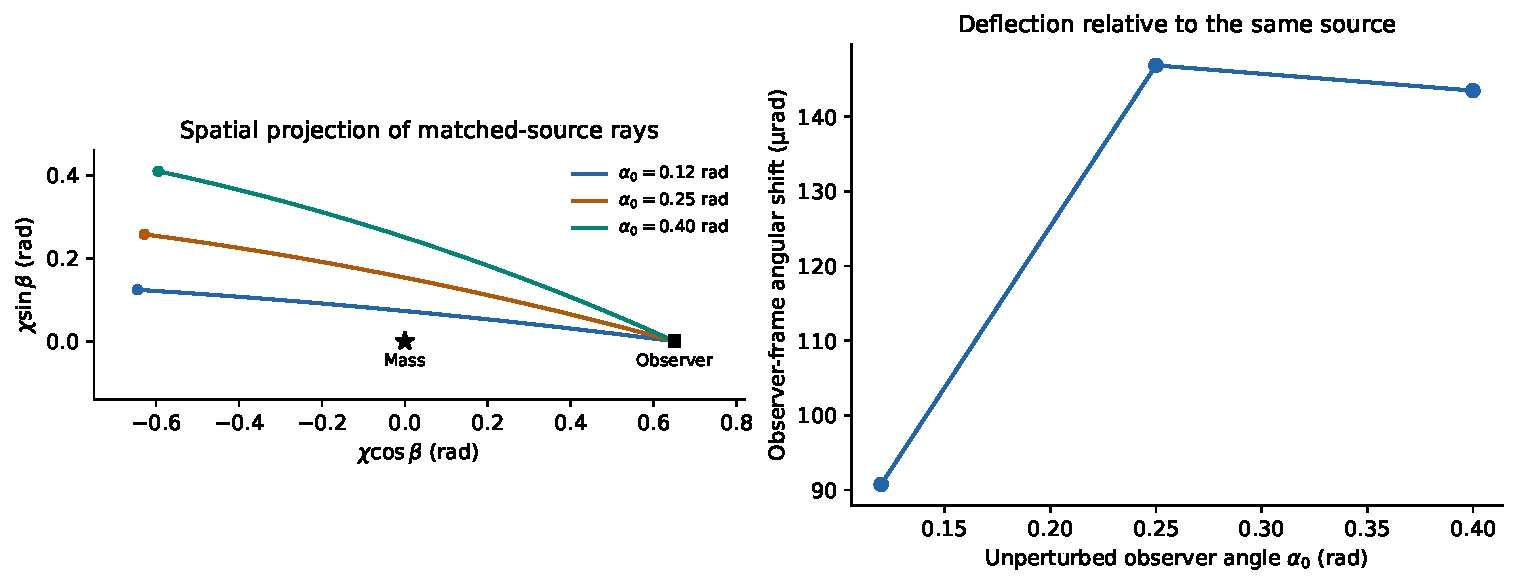
\includegraphics[width=\linewidth]{04-matched-light-rays.pdf}
 \caption{Spatial projections and observer-frame angular shifts for
 three matched sources. The left panel is a normal-coordinate drawing
 on a two-sphere section, with each dot representing its source. Physical
 deflections are too small to distinguish reliably by overplotting paths
 at this scale; the right panel reports the computed angular differences.
 The horizontal axis on the right is the baseline sky angle, not the
 temporal--radial drawing angle.}
 \label{fig:lensing}
\end{figure}
\begin{figure}[htbp]
 \centering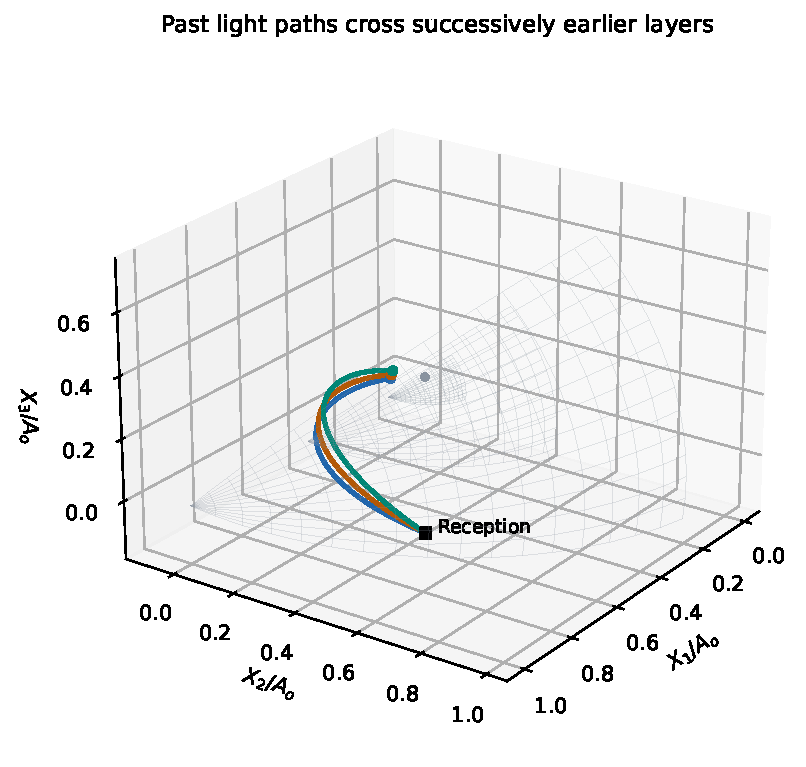
\includegraphics[width=0.78\linewidth]{05-nested-view-lines.pdf}
 \caption{The matched-source view lines in a three-coordinate section
 of the four-dimensional background embedding. Wireframes represent
 portions of the same two-sphere section at $\eta=0.65,1.2,1.8$.
 Each three-dimensional spatial universe is a three-sphere; the mesh
 shown is only a two-dimensional section of it. The radius labels time
 through $A(\eta)$, and spatial deformation is shown separately in
 Fig.~\ref{fig:deformation}. Following a line away from reception takes
 it inward through the history.}
 \label{fig:nested}
\end{figure}
\begin{figure}[htbp]
 \centering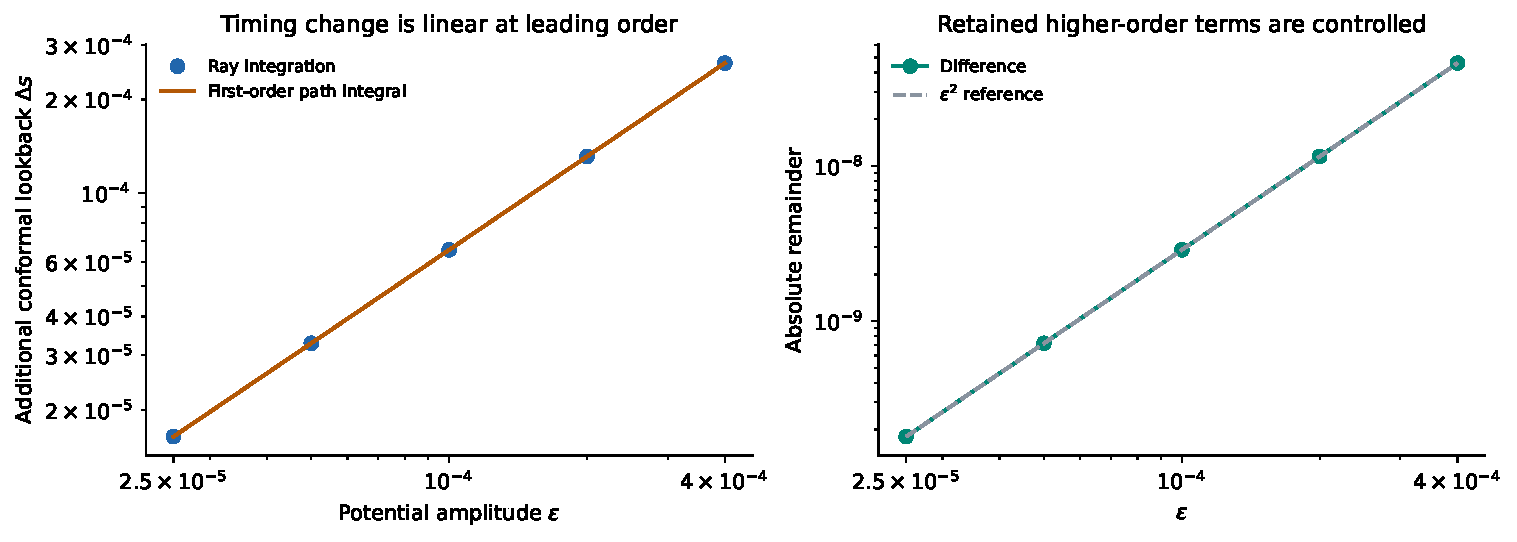
\includegraphics[width=\linewidth]{06-delay-convergence.pdf}
 \caption{Radial timing comparison and amplitude convergence. The
 difference between the integrated truncated-metric result and the
 first-order path integral scales quadratically with potential amplitude.
 This tests perturbative consistency; it does not validate missing
 second-order Einstein dynamics.}
 \label{fig:convergence}
\end{figure}

\subsection{Checks and reproducibility}
The repository contains reusable Python modules, not only figure scripts.
The numerical tests cover the background Friedmann relation, proper-time
normalization, an independent integral for the growth mode, global
compensation, the sphere Laplacian, perturbation sizes, the unperturbed
great-circle and redshift limits, ray constraints, angular-momentum
conservation, timing convergence, reflected source matching, and solver
tolerance stability. Symbolic tests check dust continuity and Euler
evolution, the closed-dust potential coefficient, the induced spatial
metric, and first-order lapse and optical-speed expansions.
Independent angular and frequency integrals also check the deflection
and the endpoint/integrated-potential contributions to redshift.

All figure files, CSV data, diagnostic JSON, and the numerical macros in
Table~\ref{tab:results} are regenerated by \texttt{make results}.
The paper is built by \texttt{make paper}, and the complete check/build
sequence by \texttt{make all}. Version pins are recorded in
\texttt{requirements.lock}; the diagnostic JSON records the scientific
package versions actually used. The default numerical parameters are
centralized in the model and reproduction script.
\FloatBarrier

\section{Interpretation, limitations, and next steps}
The view-line idea survives the addition of a consistent local perturbation.
At a fixed reception event, different directions connect the observer to
different spatial locations and earlier emission events. On the expanding
branch, those events can be drawn on progressively smaller background
layers. This is the precise meaning of ``looking inward through cosmic
history.'' It identifies a direction in the diagram's time coordinate,
not a preferred spatial direction for a telescope.

The local-mass calculation also sharpens the original picture. The
spatial deformation is controlled by $1-2\ph$, clock rates by $1+2\ph$,
and null propagation by their ratio. Their relationship comes from the
metric and field equations. It cannot be determined from the apparent
depth of an arbitrarily drawn depression. In particular, the first-order
spatial embedding has an outward core deformation and a reduced clock
rate simultaneously. A clock that accumulates less proper time remains
on a future-directed worldline; it has not moved to an earlier cosmic
slice.

The model's physical content is deliberately restricted. It is a linear
growing dust perturbation, with a specified compensation profile on a
closed background. It has no horizon and no central singularity.
Extrapolating its lapse toward zero would leave the approximation's
domain of validity. A later black-hole extension must use a suitable
strong-field metric, matter model, matching conditions, and a regular
choice of coordinates. Non-flat McVittie constructions illustrate that
embedding a mass in a closed expanding cosmology is a separate problem
with substantial global constraints \citep{Nolan2017}.

There are further representational limits. The source matching, spatial
embedding, and separated-clock comparisons are made in an explicitly
chosen gauge. Observable angles or frequency ratios require physical
observer frames; coordinate radius or timing alone is not an invariant.
Our matched-source angle uses such a frame, while the clock-offset and
conformal-delay plots retain their stated background-relative meaning.
The code's geodesics include some nonlinear dependence on a metric whose
Einstein dynamics are only linear. Amplitude scaling exposes this
distinction but does not supply the missing higher-order dynamics.

The strongest immediate use is therefore a reproducible comparison:
the same mass perturbation gives a spatial metric, a lapse, and view
lines, with their different graphical meanings kept explicit. No claim
of new cosmological dynamics or observational evidence follows. The
accompanying \emph{Comparing Cosmological Diagrams} note evaluates the
same events in four maps and identifies compression and time-folding
limits. It finds no additional physical information in the nested map;
an explanatory benefit from pairing representations remains an untested
reader-level hypothesis.

Useful next steps are to evolve emitting and receiving dust tracers,
include their Doppler terms, calculate a full angular-distance/Jacobi
map, vary curvature and background composition, and compare the weak-field
result with an exact mass-in-cosmology construction. A pedagogical study
could separately test whether readers better distinguish spatial
separation, elapsed proper time, and past-light-cone observation with
these paired diagrams.

\appendix
\section{Connection to the general FLRW visualization}
The earlier manuscript used a dimensionless scale factor $a(t_o)=1$
and a length-valued comoving radial coordinate $r$. Its radial metric is
\begin{equation}
 \dd s_{\mathrm{rad}}^2=-c^2\dd t^2+a^2(t)\dd r^2.
\end{equation}
For any positive plotting length $L$, define $R=La$ and $\psi=r/L$.
On an interval with $H>0$,
\begin{equation}\label{eq:plotting-metric}
 \dd s_{\mathrm{rad}}^2=-\frac{c^2}{H^2R^2}\dd R^2+R^2\dd\psi^2,
 \qquad \frac{\dd\psi}{\dd R}=-\frac{c}{HR^2}
\end{equation}
for an incoming future-directed ray. For a closed background with
present curvature radius $R_c$, setting $L=R_c$ gives
$R=A=R_ca$ and $\psi=\chi$. For flat or negatively curved spatial
geometry, the same polar map is a radial visualization, not a round
embedding of complete spatial slices. Changing arbitrary $L$ changes
angular sweep without changing the underlying physics.

For the illustrative history $a=(t/t_o)^p$ with $0<p<1$,
\begin{equation}
 \psi=\frac{ct_o}{L(1-p)}\left[1-(t/t_o)^{1-p}\right].
\end{equation}
The sweep is finite at the formal past limit. For $p=1$,
$\psi=(ct_o/L)\log(t_o/t)$ and the drawing is logarithmically spiral.
These shape statements are properties of the map and the chosen
history; neither implies physical rotation.

\section{Distances, horizons, and the all-sky early universe}
For a background comoving source,
\begin{equation}
 D_C=c\int_{t_e}^{t_o}\frac{\dd t}{a(t)},\qquad
 D_{\mathrm{proper}}(t)=a(t)D_C,\qquad
 1+z=\frac{1}{a(t_e)}.
\end{equation}
In a closed background, transverse comoving distance is
$D_M=R_c\sin(D_C/R_c)$ on the direct branch, and
$D_A=D_M/(1+z)$, $D_L=(1+z)D_M$ under the usual transparent-propagation
conditions \citep{Hogg1999}. These relations are background expressions;
the perturbed model requires optical transport to calculate their
direction-dependent corrections.

The particle horizon uses the convergent integral from the adopted past
boundary to reception. The event horizon uses the remaining future
integral when it converges. The Hubble radius $c/H$ is generally neither
of these causal horizons \citep{DavisLineweaver2004}.

In the thin-last-scattering background approximation, the emission
locus of the primary CMB photons received at $p_o$ is
\begin{equation}
 \mathcal S_*(p_o)=\partial J^-(p_o)\cap\Sigma_{t_*},
\end{equation}
restricted to the direct light cone before caustics. The causal past
$J^-$ itself also includes timelike-related events. The observed emission
locus samples the same early epoch in every direction; it is not a
material shell around the observer today. Finite last-scattering width,
scattering, and perturbations require a transfer calculation
\citep{SeljakZaldarriaga1996}. The geometry alone does not explain the
CMB spectrum, its near-uniformity, or the initial conditions.

\section{Numerical conventions and validity}
\begin{table}[htbp]
 \centering\small
 \begin{tabular}{@{}lp{0.72\linewidth}@{}}
 \toprule Symbol & Meaning\\\midrule
 $A$ & Length-valued background curvature radius\\
 $a$ & Dimensionless scale factor, used in the general-map appendix\\
 $\eta,s$ & Dimensionless conformal time and conformal lookback\\
 $\chi$ & Geodesic angular distance on the unit three-sphere\\
 $\alpha$ & Local observer-frame launch angle for a view line\\
 $\ph$ & Dimensionless metric potential $\Phi/c^2$\\
 $\Delta,\delta_N$ & Comoving and Newtonian-gauge density contrasts\\
 $V$ & Peculiar-velocity potential, $v^i/c=\nabla^i_\gamma V$\\
 $N,B$ & Lapse factor and conformal spatial factor of the truncated metric\\
 $\bm n,\bm p$ & Unit-sphere position and tangent optical momentum\\
 \bottomrule
 \end{tabular}
\end{table}
The default growth integration uses DOP853 with relative tolerance
$2\times10^{-12}$. Standard ray integration uses relative tolerance
$2\times10^{-10}$, checked against a tighter run. Source shooting uses
tangent-plane endpoint residuals and verifies the full embedded source
position. The numerical model checks its time interval; the example
also verifies small potential, density contrast, and peculiar velocity.
Changing width or amplitude requires rechecking all three, since a
small potential alone does not imply a linear matter perturbation.

\bibliographystyle{plainnat}
\bibliography{references}
\end{document}
